\documentclass{article}
\usepackage{amsmath}
\usepackage{amssymb}
\usepackage[colorlinks=true, allcolors=blue]{hyperref}
\usepackage{tikz}
\usetikzlibrary{fit,positioning,calc,matrix,shapes.multipart,shapes.misc,backgrounds,math}

\begin{document}

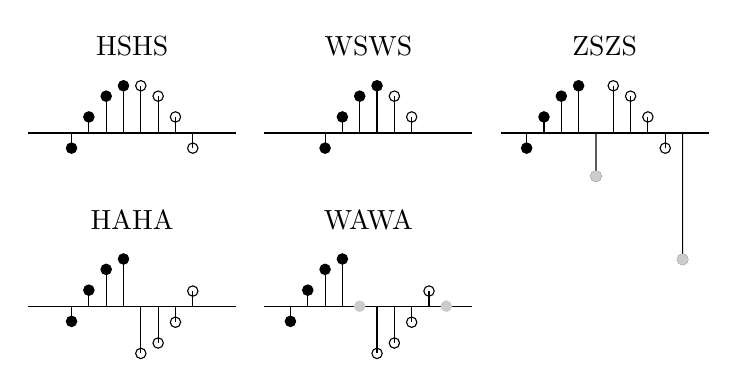
\begin{tikzpicture}

% https://tex.stackexchange.com/questions/123760/draw-crosses-in-tikz
\tikzset{cross/.style={cross out, draw, 
         minimum size=2*(#1-\pgflinewidth), 
         inner sep=0pt, outer sep=0pt}}

\tikzset{
    hshs/.pic={
        \node at (0, 5) {HSHS};
        \draw (-6, 0) -- (6, 0);
        \foreach \i in {-3.5,...,-0.5}{
            \tikzmath{\x = \i; \y = -0.3 * \x * \x + 2.8;}
            \draw[] (\x,0) -- (\x, \y);
            \draw[fill] (\x, \y) circle(0.3);
        }
        \foreach \i in {0.5,...,3.5}{
            \tikzmath{\x = \i; \xn = -\x; \y = -0.3 * \xn * \xn + 2.8;}
            \draw[] (\x,0) -- (\x,\y);
            \draw[] (\x,\y) circle(0.3);
        }
    }
}

\tikzset{
    wsws/.pic={
        \node at (0, 5) {WSWS};
        \draw (-6, 0) -- (6, 0);
        \foreach \i in {-2.5,...,0.5}{
            \tikzmath{\x = \i; \xn = \x - 1; \y = -0.3 * \xn * \xn + 2.8;}
            \draw[] (\x,0) -- (\x, \y);
            \draw[fill] (\x, \y) circle(0.3);
        }
        \foreach \i in {1.5,...,2.5}{
            \tikzmath{\x = \i; \xn = -\x; \y = -0.3 * \xn * \xn + 2.8;}
            \draw[] (\x,0) -- (\x,\y);
            \draw[] (\x,\y) circle(0.3);
        }
    }
}

\tikzset{
    zszs/.pic={
        \node at (0, 5) {ZSZS};
        \draw (-6, 0) -- (6, 0);
        \foreach \i in {-4.5,...,-1.5}{
            \tikzmath{\x = \i; \xn = \x + 1; \y = -0.3 * \xn * \xn + 2.8;}
            \draw[] (\x,0) -- (\x, \y);
            \draw[fill] (\x, \y) circle(0.3);
        }
        \tikzmath{\x = -4.5; \xn = \x + 1; \ya = -0.3 * \xn * \xn + 2.8;};
        \tikzmath{\x = -2.5; \xn = \x + 1; \yb = -0.3 * \xn * \xn + 2.8;};
        \tikzmath{\y = -2 * (\ya + \yb);};
        \draw (-0.5, 0) -- (-0.5, \y) circle(0.3);
        \draw [gray!40, fill=gray!40] (-0.5, \y) circle(0.3);
        \foreach \i in {0.5, ..., 3.5}{
            \tikzmath{\x = \i; \xn = -\x; \y = -0.3 * \xn * \xn + 2.8;}
            \draw[] (\x,0) -- (\x,\y);
            \draw[] (\x,\y) circle(0.3);
        }
        \tikzmath{\x = -3.5; \xn = \x + 1; \ya = -0.3 * \xn * \xn + 2.8;};
        \tikzmath{\x = -1.5; \xn = \x + 1; \yb = -0.3 * \xn * \xn + 2.8;};
        \tikzmath{\y = -2 * (\ya + \yb);};
        \draw (4.5, 0) -- (4.5, \y) circle(0.3);
        \draw [gray!40, fill=gray!40] (4.5, \y) circle(0.3);
    }
}

\tikzset{
    haha/.pic={
        \node at (0, 5) {HAHA};
        \draw (-6, 0) -- (6, 0);
        \foreach \i in {-3.5,...,-0.5}{
            \tikzmath{\x = \i; \xn = \x; \y = -0.3 * \xn * \xn + 2.8;}
            \draw[] (\x,0) -- (\x, \y);
            \draw[fill] (\x, \y) circle(0.3);
        }
        \foreach \i in {0.5,...,3.5}{
            \tikzmath{\x = \i; \xn = -\x; \yn = -0.3 * \xn * \xn + 2.8; \y = -\yn;}
            \draw[] (\x,0) -- (\x,\y);
            \draw[] (\x,\y) circle(0.3);
        }
    }
}

\tikzset{
    wawa/.pic={
        \node at (0, 5) {WAWA};
        \draw (-6, 0) -- (6, 0);
        \foreach \i in {-4.5,...,-1.5}{
            \tikzmath{\x = \i; \xn = \x + 1; \y = -0.3 * \xn * \xn + 2.8;}
            \draw[] (\x,0) -- (\x, \y);
            \draw[fill] (\x, \y) circle(0.3);
        }
        \draw [gray!40, fill=gray!40] (-0.5, 0) circle(0.3);
        \foreach \i in {0.5, ..., 3.5}{
            \tikzmath{\x = \i; \xn = -\x; \yn = -0.3 * \xn * \xn + 2.8; \y = -\yn;}
            \draw[] (\x,0) -- (\x,\y);
            \draw[] (\x,\y) circle(0.3);
        }
        \draw [gray!40, fill=gray!40] (4.5, 0) circle(0.3);
    }
}
\pic at (0, 0) [scale=0.22] {hshs};
\pic at (3, 0) [scale=0.22] {wsws};
\pic at (6, 0) [scale=0.22] {zszs};
\pic at (0, -2.2) [scale=0.22] {haha};
\pic at (3, -2.2) [scale=0.22] {wawa};


\end{tikzpicture}

\end{document}